%%%%%%%%%%%%%%%%%%%%%%%%%%%%%%%%%%%%%%%%%%%%%%%%%%%%%%%%%%%%%%%%%%%%%%%%%%%%%%%%
%2345678901234567890123456789012345678901234567890123456789012345678901234567890
%        1         2         3         4         5         6         7         8

\documentclass[letterpaper, 10 pt, conference]{ieeeconf}  % Comment this line out if you need a4paper

%\documentclass[a4paper, 10pt, conference]{ieeeconf}      % Use this line for a4 paper

\IEEEoverridecommandlockouts                              % This command is only needed if 
                                                          % you want to use the \thanks command

\overrideIEEEmargins                                      % Needed to meet printer requirements.

%In case you encounter the following error:
%Error 1010 The PDF file may be corrupt (unable to open PDF file) OR
%Error 1000 An error occurred while parsing a contents stream. Unable to analyze the PDF file.
%This is a known problem with pdfLaTeX conversion filter. The file cannot be opened with acrobat reader
%Please use one of the alternatives below to circumvent this error by uncommenting one or the other
%\pdfobjcompresslevel=0
%\pdfminorversion=4

% See the \addtolength command later in the file to balance the column lengths
% on the last page of the document

% The following packages can be found on http:\\www.ctan.org
\usepackage{graphics} % for pdf, bitmapped graphics files
\usepackage{epsfig} % for postscript graphics files
\usepackage{times} % assumes new font selection scheme installed
\usepackage{amsmath} % assumes amsmath package installed
\usepackage{amssymb}  % assumes amsmath package installed
\usepackage{svg}
\usepackage{graphicx}
\usepackage{listings}
\usepackage{xcolor}
\usepackage{booktabs}
\usepackage{url}
\usepackage{placeins} % \FloatBarrier -- keeps figures from drifting past the References section

\newcommand{\zz}[1]{{\color{red}ZZ: #1}}

\title{\LARGE \bf
Graph-Guided Long-Horizon Robotic Assembly via Vision-Language Reasoning and Logic-Geometric Programming}


\author{Anonymous Authors% <-this % stops a space
% \thanks{*This work was not supported by any organization}% <-this % stops a space
% \thanks{$^{1}$Albert Author is with Faculty of Electrical Engineering, Mathematics and Computer Science,
%         University of Twente, 7500 AE Enschede, The Netherlands
%         {\tt\small albert.author@papercept.net}}%
% \thanks{$^{2}$Bernard D. Researcheris with the Department of Electrical Engineering, Wright State University,
%         Dayton, OH 45435, USA
%         {\tt\small b.d.researcher@ieee.org}}%
}

\begin{document}

\maketitle
\thispagestyle{empty}
\pagestyle{empty}


\begin{abstract}

\end{abstract}


\section{Introduction}

Long-horizon multi-part robotic assembly is a fundamental capability for intelligent manufacturing and embodied robotics, with broad applications in both industrial production and daily household environments~\cite{li2019survey,daneshmand2023industry,zhu2018robot}. 
Unlike single-step manipulation, these tasks require the robot to accomplish a sequence of interdependent assembly operations while satisfying task dependencies and physical constraints~\cite{jiang2022review}. 
Automating such processes could greatly expand the practical deployment of robotic assembly systems by reducing manual programming effort and improving adaptability to diverse tasks. 
However, achieving autonomous long-horizon assembly remains challenging, as the robot must accurately infer the assembly objective, generate a logically consistent task plan, and produce physically feasible motions for each assembly step~\cite{faccio2019collaborative}. 
Moreover, the tight coupling between high-level task planning and low-level motion planning, together with the long-term dependencies across assembly decisions, further increases the complexity of reliable autonomous assembly~\cite{garrett2021integrated}.

Classical approaches to long-horizon robotic assembly are primarily built on model-based Task and Motion Planning (TAMP)~\cite{zhao2024survey,guo2023recent}, which typically employs symbolic planners, such as those based on Planning Domain Definition Language (PDDL)~\cite{aeronautiques1998pddl,jiang2019task}, to generate task plans, followed by motion planners to compute feasible trajectories for each action.
A representative TAMP approach is Logic-Geometric Programming (LGP)~\cite{marc2015LGP}, which integrates task planning and motion planning into a unified optimization framework, allowing motion feasibility to be considered during task planning rather than as a separate step.
By explicitly modeling task semantics and constraints, these methods produce interpretable and verifiable planning results~\cite{toussaint2017multi}. 
However, they heavily rely on manually specified task definitions, object models, and action rules, requiring substantial engineering effort and domain expertise. 
Consequently, extending these methods to new objects or assembly objectives often needs manual redesign of symbolic models and planning rules, limiting their scalability and adaptability to diverse real-world scenarios.

Recently, Large Language Models (LLMs) have been introduced to robotic assembly to improve high-level task understanding and planning~\cite{gkournelos2024llm,ao2025llm}. 
By leveraging their reasoning capabilities, LLMs are able to directly interpret human instructions, infer assembly intent, and generate task plans without manually defined symbolic specifications~\cite{zhou2024isr}. 
This capability greatly reduces engineering effort and improves adaptability to diverse tasks, thereby enabling more flexible robotic assembly systems in changing environments. 
However, the generated task plans are not guaranteed to be logically correct or physically executable, as LLMs lack reliable reasoning over kinematic constraints and motion feasibility~\cite{wang2025large}. 
Another practical limitation is that most existing LLM-based approaches assume natural language instructions as input~\cite{qi2026llm}, whereas many real-world assembly tasks, particularly in industrial settings, are specified by target assembly images rather than textual descriptions.

In this work, we aim to realize autonomous long-horizon robotic assembly directly from a target assembly image while ensuring safe and reliable motion execution. 
To this end, we propose a unified framework that combines the visual reasoning capability of Vision-Language Models (VLMs) with the optimization-based guarantees of LGP. 
Given a target assembly image and the current scene, the framework infers the assembly goal, identifies the required object components, determines an appropriate assembly sequence, and generates executable robot motions that satisfy kinematic and dynamic constraints (see Fig.~\ref{fig:workflow}). 
Specifically, it consists of three key components: 
(1) \textit{VLM-Based Task Understanding}: the VLM first interprets the target assembly image to construct an assembly graph, from which assembly action plans are derived through graph decomposition and clustering; 
(2) \textit{Reachability-Manipulability-Aware Scene Understanding}: the robot then perceives the workspace, identifies the corresponding manipulatable objects, and prioritizes them according to reachability and manipulability; 
(3) \textit{LGP-Based Motion Execution}: finally, the derived task plan and scene information are integrated into an LGP to produce collision-free and physically feasible motion trajectories for completing the assembly task. 
Note that, the computational complexity of LGP increases rapidly with the number of objects, making its direct usage in long-horizon assembly problems impractical. 
To address this issue, we decompose the overall assembly process into a sequence of short-horizon subtasks during the VLM-based task understanding, and introduce an active-constraint LGP formulation to further improve computational efficiency.



\zz{add experiments and results descriptions} 
We evaluate our methods on... 
The results show that...

\zz{add contributions}
Our main contributions are threefold:
\begin{itemize}
    \item A constrained VLM interface for extracting an assembly representation from a target image;
    \item A formal, precedence-preserving decomposition that produces solver-bounded LGP subproblems;
    \item An end-to-end evaluation of graph quality, planning scalability, and physical execution.
\end{itemize}

\section{Related Work}

\zz{to add references and check content later}


\subsection{Assembly Sequence Planning and Structural Representations}

Assembly Sequence Planning (ASP) is typically defined as the process of transforming the final target structure into a series of executable component assembly operations.
Classic ASP research typically employs graph structures to represent feasible assembly sequences, constraint relationships, and sub-assembly states.
Typical methods include precedence graphs, contact graphs, support graphs, and AND/OR graphs.
There are also graph decomposition methods for construction and stacking tasks.
The priority graph is typically used to represent sequential constraints between different assembly operations.
The contact graph and connection graph are used to describe physical contact, connection, or interference relationships between parts.
The support graph further considers factors such as gravity, load-bearing capacity, and the stability of intermediate structures.
The AND/OR graph decomposes assembly tasks into multiple intermediate structures, thereby reducing search complexity.
For building construction and block-stacking tasks, the graph decomposition method is often combined with stability constraints to ensure that the intermediate structures generated at each step are physically feasible.

In recent years, the input formats for assembly tasks have expanded from traditional CAD models to include images, instruction manuals, and multi-modal instructions.
However, most methods still rely on known geometric models, predefined part relationships, manually designed support relationships, or assembly instructions that already contain step information.
In other words, existing methods typically assume that assembly relationships are already given, rather than deriving usable structures directly from visual information.
Unlike these methods, the system proposed in this paper extracts a structured representation from target images for LGP solving.
LGP transforms the target assembly state in the image into an input containing symbolic relationships and geometric constraints.
This bridges the gap between visual task descriptions and executable autonomous assembly planning.

\subsection{Task and Motion Planning for Long-Horizon Assembly}
Long-horizon assembly tasks can typically be modeled as Task and Motion Planning (TAMP) problems, in which discrete assembly decisions and continuous robot motion must be considered together.
In integrated TAMP frameworks such as LGP, symbolic task selection and geometric motion constraints are solved through a unified optimization process.
LGP is a typical TAMP formulation method that combines discrete logic programming with continuous trajectory optimization.
Since the feasibility of assembly operations depends not only on logical order but is also influenced by constraints such as reachability, stability, and contact relationships, LGP is suitable for describing complex assembly tasks.
However, when assembly tasks involve multiple objects and long sequences of operations, directly solving the LGP problem leads to a rapid expansion of the search space.

To improve the scalability of long-horizon LGP, existing research typically employs methods such as hierarchical LGP, receding-horizon LGP, heuristic search, and subproblem decomposition.
These methods can reduce the scale of a single solution.
However, fixed-horizon may overlook object dependencies and support relationships within the assembly.
And the receding-horizon method may lack global structural information and require frequent re-planning.
The decomposition method proposed in this paper is not based on the fixed-horizon but rather divides the task according to the assembly structure inferred from the target image.
By extracting object relationships, support dependencies, and sub-assemblies, this structural information is defined as individual LGP subproblems.
The method proposed in this paper preserves the global assembly intent while keeping the subproblems simple.

\subsection{Foundation Models in Robotic Assembly}
Foundational models have been widely adopted in robotic manipulation and assembly tasks to enhance task understanding and long-term planning capabilities.
Some studies utilize Large Language Models (LLM) to generate high-level task plans based on natural language instructions.
Other studies utilize Visual-Language Models (VLM) to identify objects in images, infer spatial relationships, and generate assembly steps.
Furthermore, Visual-Language-Action (VLA) models attempt to directly map visual observations and language instructions to robotic actions, thereby enabling end-to-end manipulation control.
While these methods enhance task understanding and action generation, they lack an explicit representation of geometric feasibility, contact constraints, support dependencies, and stability conditions in long-term assembly tasks.

To improve reliability, many studies adopt modular systems that combine LLM/VLM with classical planners, linking perception and planning through scene graphs, object relationships, and constraints.
Compared to free-form text, this type of structured output is better suited for robotic execution.
However, most existing methods are designed for general scene understanding and are not specifically optimized for tasks and motion planners based on LGP.
The VLM proposed in this paper outputs a constrained representation of assembly relationships, extracting information directly from target images.
And converts it into input for LGP.
Therefore, this paper does not directly generate actions using the VLM.
This paper uses the VLM to establish an interface between visual target descriptions and LGP long-time-domain assembly planning.


% \subsection{Assembly Sequence Planning and Structural Representations}

% Topics to cover (follow the sequence of autonomous assembly, cover them one by one):
% - precedence graphs
% - contact and support graphs
% - subassembly generation
% - assembly ordering, which also covers stability constraints/considerations
% - graph decomposition for construction and stacking
% - assembly specified by image, CAD, instruction, etc.

% The review of literature should converge to the message i.e. existing structural representations generally assume a known geometric model or predefined relations; our proposed system derives a solver-oriented (i.e., LGP) structure from a target image.

% \subsection{Task and Motion Planning for Long-Horizon Assembly}

% Cover in this subsection:

% - integrated TAMP
% - LGP and KOMO
% - receding-horizon or hierarchical LGP
% - heuristic search reduction
% - reachability-guided planning
% - subproblem decomposition in construction and assembly

% The comparison with literature must clarify how the proposed decomposition differs from: (1) generic fixed-horizon, or (2) receding-horizon approaches.

% \subsection{Foundation Models in Robotic Assembly}

% Cover:
% - LLM-generated plans
% - VLM-based scene + task reasoning
% - direct visuomotor or VLA methods
% - modular systems, e.g., VLM + planner
% - structured outputs, e.g., scene graphs, constraints, and sub-goals

% This review should point out the gap in the literature:
% our proposed VLM produces a constrained assembly relation representation specifically designed for downstream LGP


\section{Problem Formulation}
\label{sec:problem_formulation}

We consider the problem of accomplishing long-horizon robotic assembly directly from a target image, without relying on manually specified symbolic task descriptions. 
The input consists of a target assembly image $\mathcal{I}$ and the current scene information $\mathcal{S}=\{o_1,\dots,o_N\}$, where each object instance $o_i$ is characterized by its pose and geometric attributes. 
To achieve image-based autonomous assembly, the following key problems should be addressed:

\begin{itemize}
\item First, the target assembly image $\mathcal{I}$ needs to be transformed into a structured representation that captures the desired configuration and enables action sequence generation. 
In this work, we employ an assembly graph $\mathcal{G}= (\mathcal{V},\mathcal{E})$, obtained as
\begin{equation}
\mathcal{G} = f_{\mathrm{G}}(\mathcal{I}),
\label{eq:problem_goal}
\end{equation}
where $f_{\mathrm{G}}$ denotes the image-to-graph conversion. 
Each node $v\in\mathcal{V}$ represents an object instance, while each directed edge $(u,v)\in\mathcal{E}$ specifies that object $u$ should be connected to object $v$ as a supporting component.
\item Second, a high-level task plan $\mathcal{P}$ needs to be derived from the assembly graph $\mathcal{G}$, specifying the sequence of assembly actions and the order in which individual objects should be assembled.
\item Lastly, the task plan $\mathcal{P}$ needs to be translated into executable robot motions based on the current scene $\mathcal{S}$. 
This involves selecting the appropriate object for each assembly action and generating collision-free, physically feasible motion trajectories that satisfy the robot's kinematic and dynamic constraints.
\end{itemize}

%The first problem is to determine the assembly goal from $\mathcal{I}$. 
%We represent this goal as an object-support graph $\mathcal{G}=(\mathcal{V},\mathcal{E})$, where each node $v\in\mathcal{V}$ denotes one target object instance and each directed edge $(u,v)\in\mathcal{E}$ denotes that object $u$ must support object $v$ in the completed assembly:

% The second problem is to determine a task plan $\mathcal{P}$ for realizing $\mathcal{G}$. 

% We represent $\mathcal{P}=(B_1,\dots,B_M)$ as an ordered sequence of $M$ execution batches, in which every node of $\mathcal{V}$ appears in exactly one batch, each batch respects a solver-imposed size bound, and every node in $B_m$ has all of its supporters already placed in an earlier batch $B_1,\dots,B_{m-1}$:
% \begin{equation}
%   \mathcal{P} = f_{\mathrm{decomp}}(\mathcal{G}).
%   \label{eq:problem_plan}
% \end{equation}

% The third problem is to associate $\mathcal{G}$ and $\mathcal{P}$ with the current scene $\mathcal{S}$, i.e., to determine which concrete object instance should be used to realize each node $v\in\mathcal{V}$. 
% This requires a grounding map $\pi:\mathcal{V}\to\mathcal{S}_{\mathrm{feas}}$, where $\mathcal{S}_{\mathrm{feas}}\subseteq\mathcal{S}$ is the subset of instances that are kinematically reachable, and $\pi$ additionally prefers instances that are easier for the robot to manipulate.

% Finally, for each grounded batch $\pi(B_m)$, the system must determine a collision-free, physically feasible motion trajectory $x_m^\ast$ that realizes the corresponding support relations under the kinematic and dynamic constraints of the robot. 

% The overall problem is therefore to find
% \begin{equation}
%   \mathcal{G},\quad \mathcal{P},\quad \pi,\quad \{x_m^\ast\}_{m=1}^{M}
%   \label{eq:problem_all}
% \end{equation}
% such that executing $\{x_m^\ast\}_{m=1}^{M}$ on the physical robot yields a final scene configuration consistent with the support relations specified by $\mathcal{G}$.


\section{Method}
\begin{figure*}[!t]
\centering
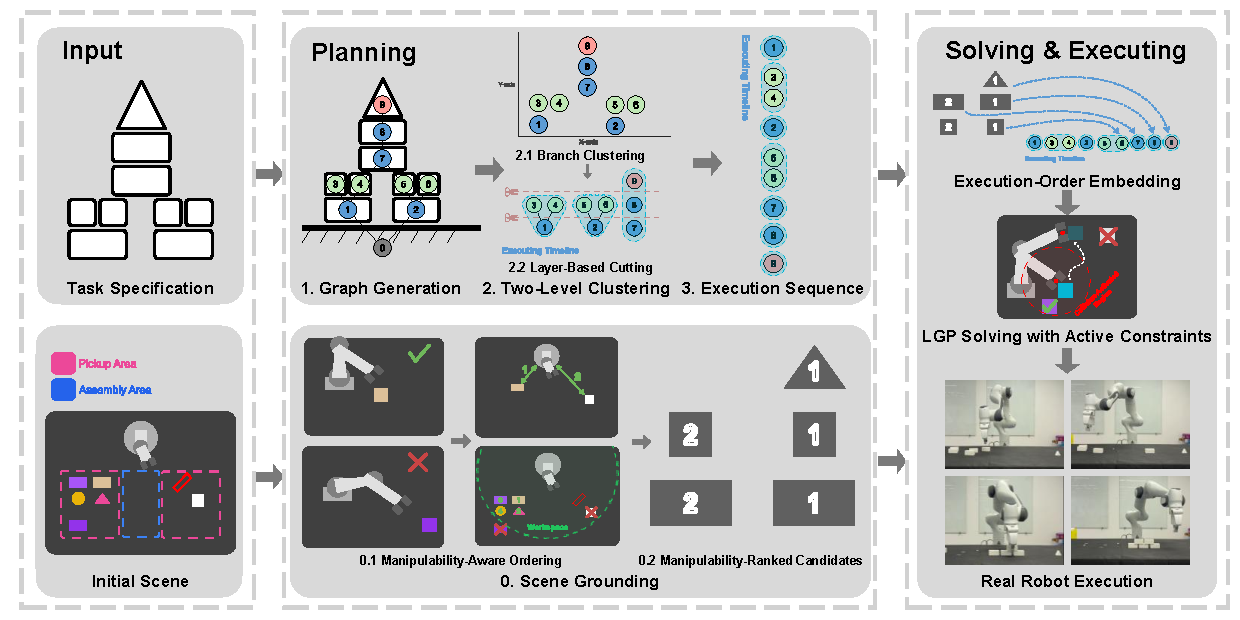
\includegraphics[width=\textwidth]{figures/LGP_method.pdf}
\caption{The overall workflow of the proposed VLM-LGP framework.}
\label{fig:workflow}
\end{figure*}

% This section presents the proposed framework for accomplishing long-horizon robotic assembly from a target assembly image.
As illustrated in Fig.~\ref{fig:workflow}, the framework consists of three components. 
First, a VLM analyzes the target assembly image to construct an assembly graph and generate a sequence of assembly actions (Sec.~\ref{sec:task_understanding}). 
Second, the robot perceives the workspace to identify the corresponding objects and prioritize them according to reachability and manipulability (Sec.~\ref{sec:scene_understanding}). 
Finally, the task plan and scene information are integrated into a LGP formulation to produce feasible motions for each assembly step (Sec.~\ref{sec:motion_execution}). 

\zz{write the method corresponding to the outline given in the last paragraph of the introduction, we have three components, detail each one in one subsection}

\subsection{VLM-Based Task Understanding}
\label{sec:task_understanding}

\zz{Introduce in each subsubsection: 1. how VLM converts the image input into assembly graph. 2. How this graph is converted into action plans}

\subsubsection{VLM for Assembly Graph Generation}
\textcolor{red}{Input: Image, Output: Graph}

Following the mapping $\mathcal{G}=f_{\mathrm{VLM}}(\mathcal{I})$ introduced in
Section~\ref{sec:problem_formulation}, we use a VLM to convert the target
assembly image $\mathcal{I}$ into the object-support graph
$\mathcal{G}=(\mathcal{V},\mathcal{E})$, rather than asking it to predict
precise object coordinates or a long executable program directly. This
choice follows the capability boundary of current VLMs: they are
comparatively reliable at inferring relational structure, support
dependencies, and coarse left-right or above-below organization, but less
stable when required to output exact geometry, long symbolic code, or
mathematically precise layouts. We therefore let the VLM produce the
structural representation that it is best suited to provide. Each node
$v \in \mathcal{V}$ denotes one target object instance, and each directed
edge $(u,v) \in \mathcal{E}$ indicates that object $u$ must support object
$v$ in the final assembly. The graph is directed because support precedence
is asymmetric, and optional local labels such as left/right placement hints
are retained only as geometric side information rather than as the
execution order itself.

\subsubsection{Graph Decomposition and Clustering}
\textcolor{red}{Input: Graph, Output: Short-horizon action plans}

Following the mapping $\mathcal{P}=f_{\mathrm{decomp}}(\mathcal{G})$
introduced in Section~\ref{sec:problem_formulation}, this step converts the
support graph $\mathcal{G}$ into the task plan
$\mathcal{P}=(B_1,\dots,B_M)$, i.e., a precedence-consistent sequence of
short-horizon execution batches. Exposing the full graph to the solver at
once is impractical, whereas placing objects strictly one at a time is
unnecessarily slow; the decomposition must also respect support precedence,
so that no object is scheduled before all of its supporters. We therefore
compute $f_{\mathrm{decomp}}$ in two stages that operate directly on
$\mathcal{G}$: a coarse branch grouping followed by a per-branch cutting
into solver-sized batches.

The first stage, \emph{branch-based grouping}, identifies the coarse
structural organization of $\mathcal{G}$. We assign each node $v$ a layer
number by propagating outward from the table root, which is fixed to
layer~$0$:
\begin{equation}
  \mathrm{layer}(v) =
  \begin{cases}
    0, & \mathrm{supporters}(v)=\varnothing,\\[2pt]
    1 + \displaystyle\max_{u \in \mathrm{supporters}(v)} \mathrm{layer}(u), & \text{otherwise,}
  \end{cases}
  \label{eq:layer}
\end{equation}
where $\mathrm{supporters}(v)$ is the set of nodes with a direct edge into
$v$; only the table root has no supporters, so every object resting on the
table has layer~$1$. Each layer-$1$ node is assigned to a branch according
to the placement label (e.g., left/right) of its table support, and this
branch label is propagated to higher layers along the support edges; a node
whose supporters belong to two or more distinct branches is instead assigned
to a dedicated \emph{bridge} branch. This stage groups $\mathcal{V}$ into a
small number of branches without yet committing to an execution order.

The second stage, \emph{layer-based cutting}, turns the grouped graph into
the ordered batch sequence $\mathcal{P}$. The branches are first ordered so
that a branch is cut only after every branch it depends on, through
cross-branch support edges, has already been scheduled. Each branch is then
cut independently: its nodes are processed in increasing support depth, and
at each depth the nodes sharing the same in-branch supporter set
\begin{equation}
  r(v) = \{\, u \in \mathrm{supporters}(v) : \mathrm{branch}(u)=\mathrm{branch}(v) \,\}
  \label{eq:role}
\end{equation}
are collected, ordered by node identifier for a deterministic result, and
split into batches of at most $B_{\max}=2$ nodes. Concatenating the batches
of all branches in order yields $\mathcal{P}$. For a nine-object assembly
with three independent branches (objects $1,3,4$; $2,5,6$; $7,8,9$), this
procedure yields
\begin{equation}
  \mathcal{P} = \big(\{1\},\{3,4\},\{2\},\{5,6\},\{7\},\{8\},\{9\}\big),
  \label{eq:plan_example}
\end{equation}
where each set is one execution batch $B_m$ submitted to the solver. The
batch bound $B_{\max}=2$ reflects the scale at which the downstream solver
remains efficient under our hardware constraints.

\subsection{Reachability-Manipulability-Aware Scene Understanding}
\label{sec:scene_understanding}

\zz{Introduce in each subsubsection: 1. how reachability is considered. 2. How manipulability is used to order the list of the manipulable objects}

\subsubsection{Reachability Filtering}
\textcolor{red}{Input: Scene Information, Output: Reachability filtered list of objects}

This step takes the current scene $\mathcal{S}=\{o_1,\dots,o_N\}$ introduced
in Section~\ref{sec:problem_formulation} and returns the subset
$\mathcal{S}_{\mathrm{feas}}\subseteq\mathcal{S}$ of object instances that
the robot can actually reach. We apply two successive filters: a cheap
geometric prior that discards obviously inaccessible objects, followed by a
rigorous kinematic check on the survivors.

The first filter assigns each object a scalar geometric score $\rho(o_i)$
based on its position relative to the surrounding scene geometry, combining a
density term $\rho_{\mathrm{gmm}}$ and a clearance term $\rho_{\mathrm{esdf}}$.
The density term is a Gaussian kernel of bandwidth $\sigma = 0.12\,\mathrm{m}$
evaluated over the pick points of all objects in $\mathcal{S}$:
\begin{equation}
  \rho_{\mathrm{gmm}}(o_i) = \frac{1}{N} \sum_{j=1}^{N}
    \exp\!\left(-\frac{\|p_i - p_j\|^2}{2\sigma^2}\right),
  \label{eq:reach_gmm}
\end{equation}
where $p_i$ is the pick point of object $o_i$ (the handle sub-frame center
if available, otherwise the geometric center), and a higher value indicates
that $o_i$ lies in a geometrically central, more accessible region. The
clearance term measures the distance to surrounding obstacles, each
approximated as a bounding sphere with center $c_k$ and radius $r_k$:
\begin{equation}
  \rho_{\mathrm{esdf}}(o_i) = \min_k \frac{\max\!\left(0,\ \min\!\left(\|p_i - c_k\| - r_k,\ d_{\max}\right)\right)}{d_{\max}},
  \label{eq:reach_esdf}
\end{equation}
with $d_{\max} = 0.20\,\mathrm{m}$, so that a higher value indicates more
open space around the object. The two terms are linearly combined into the
geometric score,
\begin{equation}
  \rho(o_i) = \alpha \, \rho_{\mathrm{gmm}}(o_i) + \beta \, \rho_{\mathrm{esdf}}(o_i),
  \qquad \alpha = 0.6,\ \beta = 0.4,
  \label{eq:reach_fused}
\end{equation}
and an object passes this filter if $\rho(o_i) \geq \tau_r = 0.45$.

The second filter verifies kinematic feasibility on the objects that survive
the geometric prior. For each such candidate $o_i$, we construct a
single-step KOMO subproblem $\Pi_i^{\mathrm{pick}}$ that asks the solver to
find a robot configuration from which a grasp of $o_i$ can be initiated,
using the same KOMO/RAI framework and the full set of kinematic and
collision constraints as the main solver. The object is retained only if
this subproblem is feasible:
\begin{equation}
  \mathrm{Reach}(o_i) =
  \mathbb{I}\!\left[\mathrm{Feasible}\!\left(\Pi_i^{\mathrm{pick}}(o_i)\right)\right].
  \label{eq:reach_check}
\end{equation}
The two filters are complementary: the geometric prior removes clearly
unreachable objects at negligible cost, while the pick-waypoint check
provides rigorous verification only where it is needed. The output is the
reachable subset
$\mathcal{S}_{\mathrm{feas}} = \{\, o_i \in \mathcal{S} : \rho(o_i)\ge\tau_r \ \wedge\ \mathrm{Reach}(o_i)=1 \,\}$,
which is passed to the ordering step below.

\begin{figure*}[!t]
  \centering
  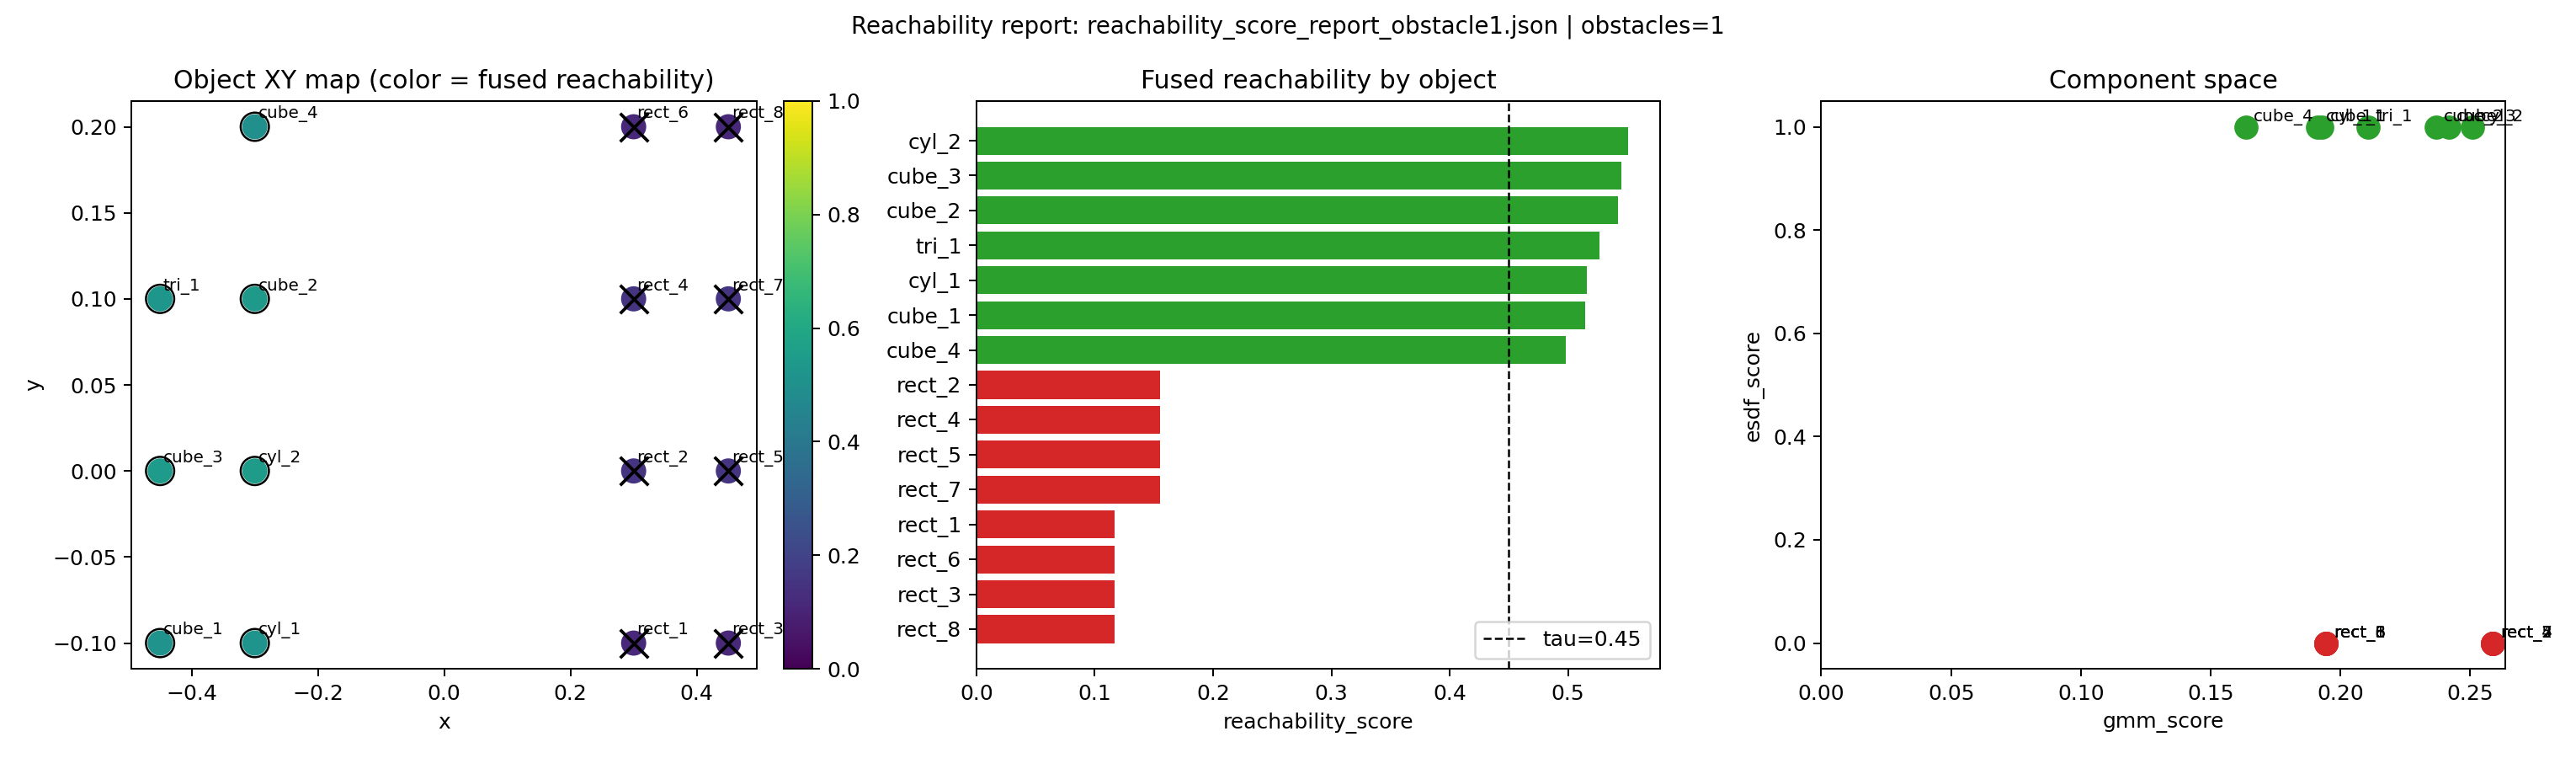
\includegraphics[width=\textwidth]{figures/Reachability.png}
  \caption{Reachability screening result: objects passing both the geometric prior and the pick-waypoint feasibility check are retained, while remaining candidates are pruned before downstream LGP solving.}
  \label{fig:reachability}
\end{figure*}

\subsubsection{Manipulability-Aware Object Ordering}
\textcolor{red}{Input: Reachability filtered list of object, Output: Manipulability ordered list of objects}

This step takes the reachable subset $\mathcal{S}_{\mathrm{feas}}$ and
orders its instances by how comfortably the robot arm can approach them, so
that the grounding map $\pi$ of Section~\ref{sec:problem_formulation} can
prefer easier-to-manipulate instances. For each object
$o_i \in \mathcal{S}_{\mathrm{feas}}$, we define an approach target slightly
above the object, solve a damped least-squares inverse kinematics problem
for that target, and evaluate the positional Yoshikawa manipulability score
at the resulting configuration $q_i$:
\begin{equation}
  m(o_i) = \sqrt{\det\!\left(J_p(q_i)\,J_p(q_i)^\top\right)},
  \label{eq:manip}
\end{equation}
where $J_p(q_i)$ is the position Jacobian of the robot at $q_i$. A higher
$m(o_i)$ indicates a more dexterous approach configuration. Within each
object category, instances are ranked by decreasing $m(o_i)$, and instances
whose inverse kinematics fails are placed last. The output is thus, for each
category, a manipulability-ordered list of reachable instances; this
ordering defines the preference that the grounding map $\pi$ uses to select
a concrete instance when a batch requires an object of that category.

\begin{figure*}[!t]
  \centering
  \setlength{\tabcolsep}{2pt}
  \begin{tabular}{@{}cccc@{}}
    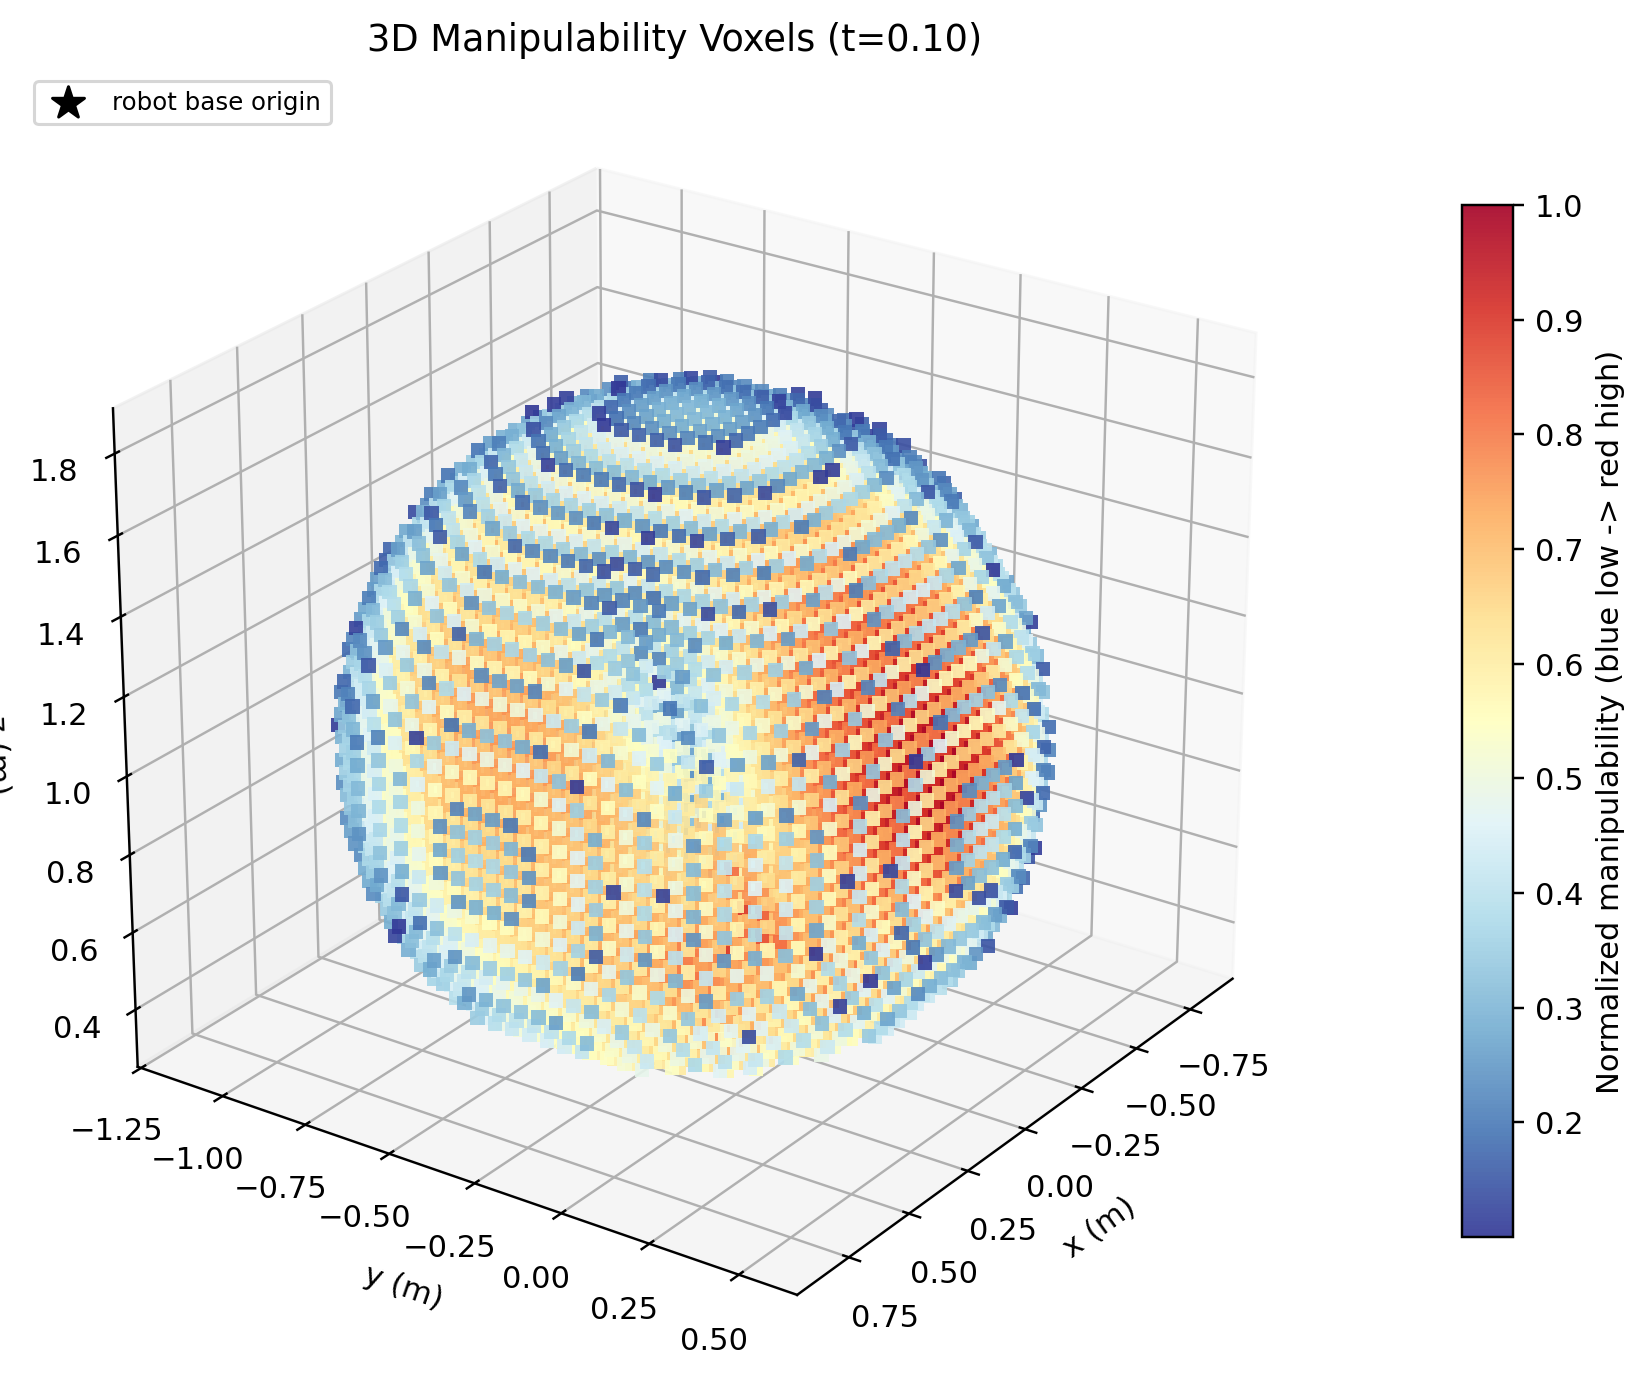
\includegraphics[width=0.24\textwidth]{figures/Manipulability_1.png} &
    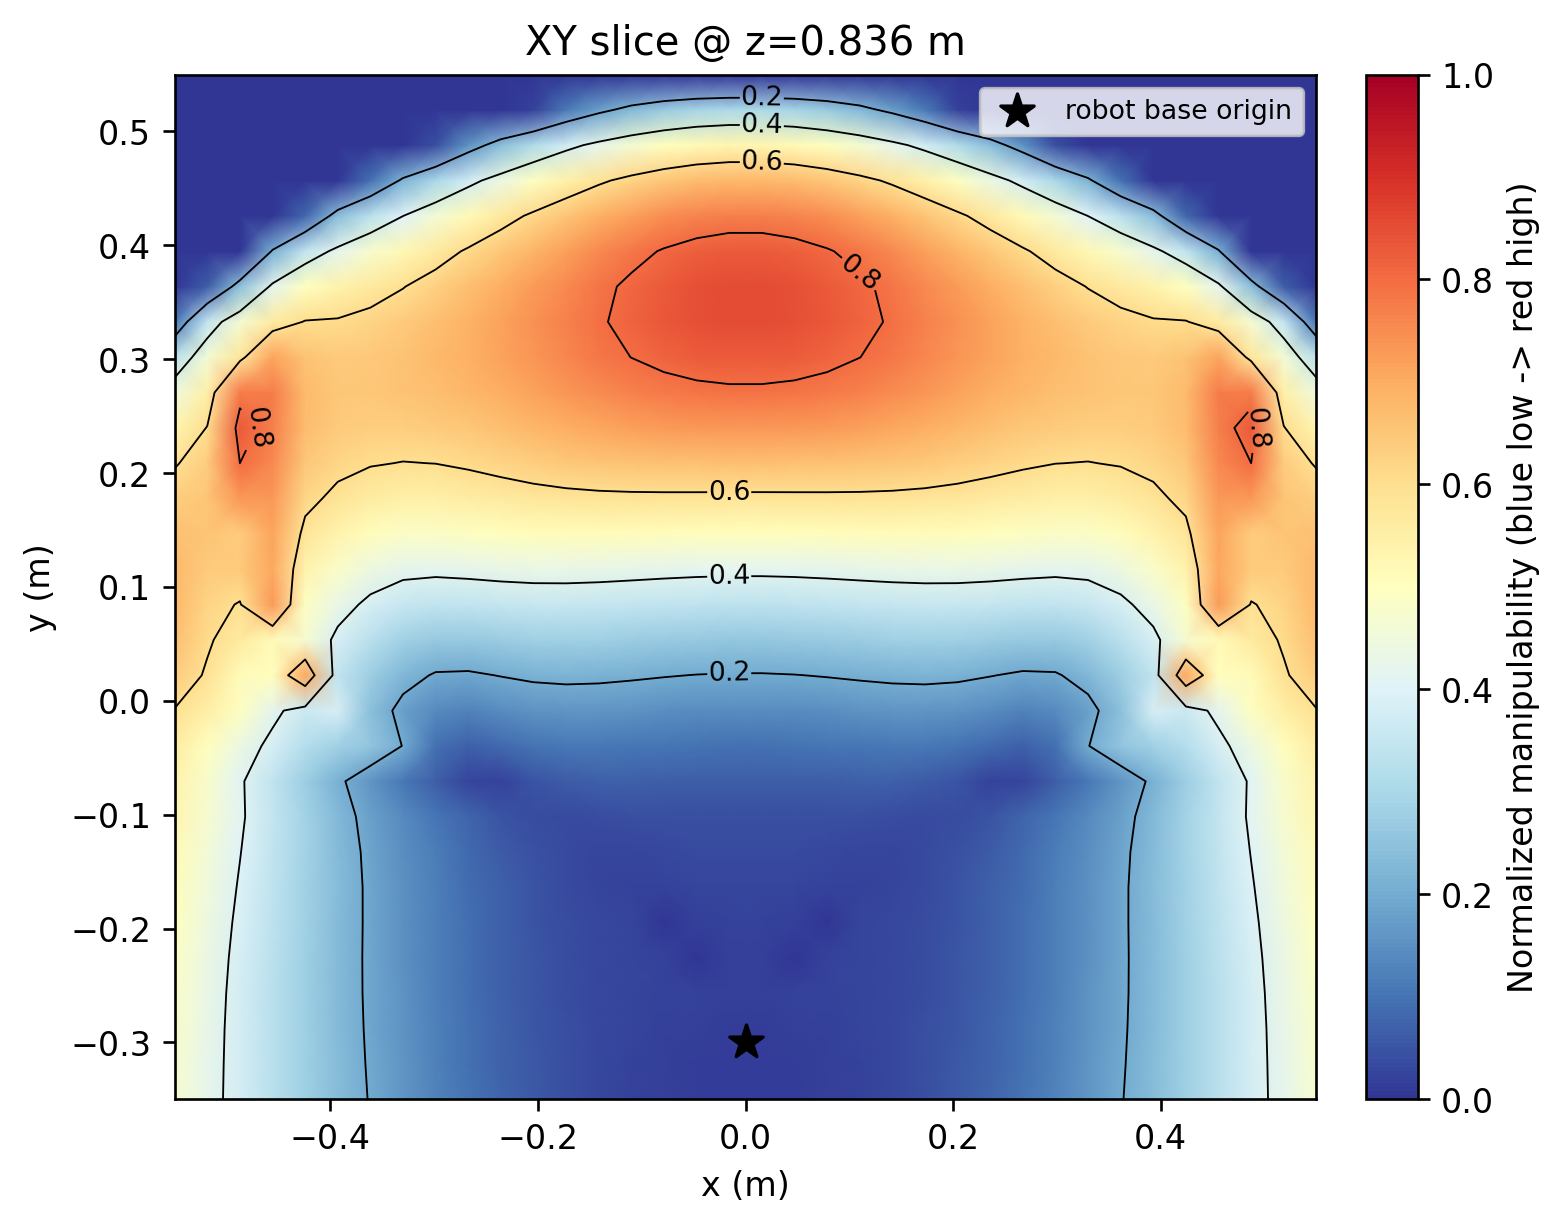
\includegraphics[width=0.24\textwidth]{figures/Manipulability_2.png} &
    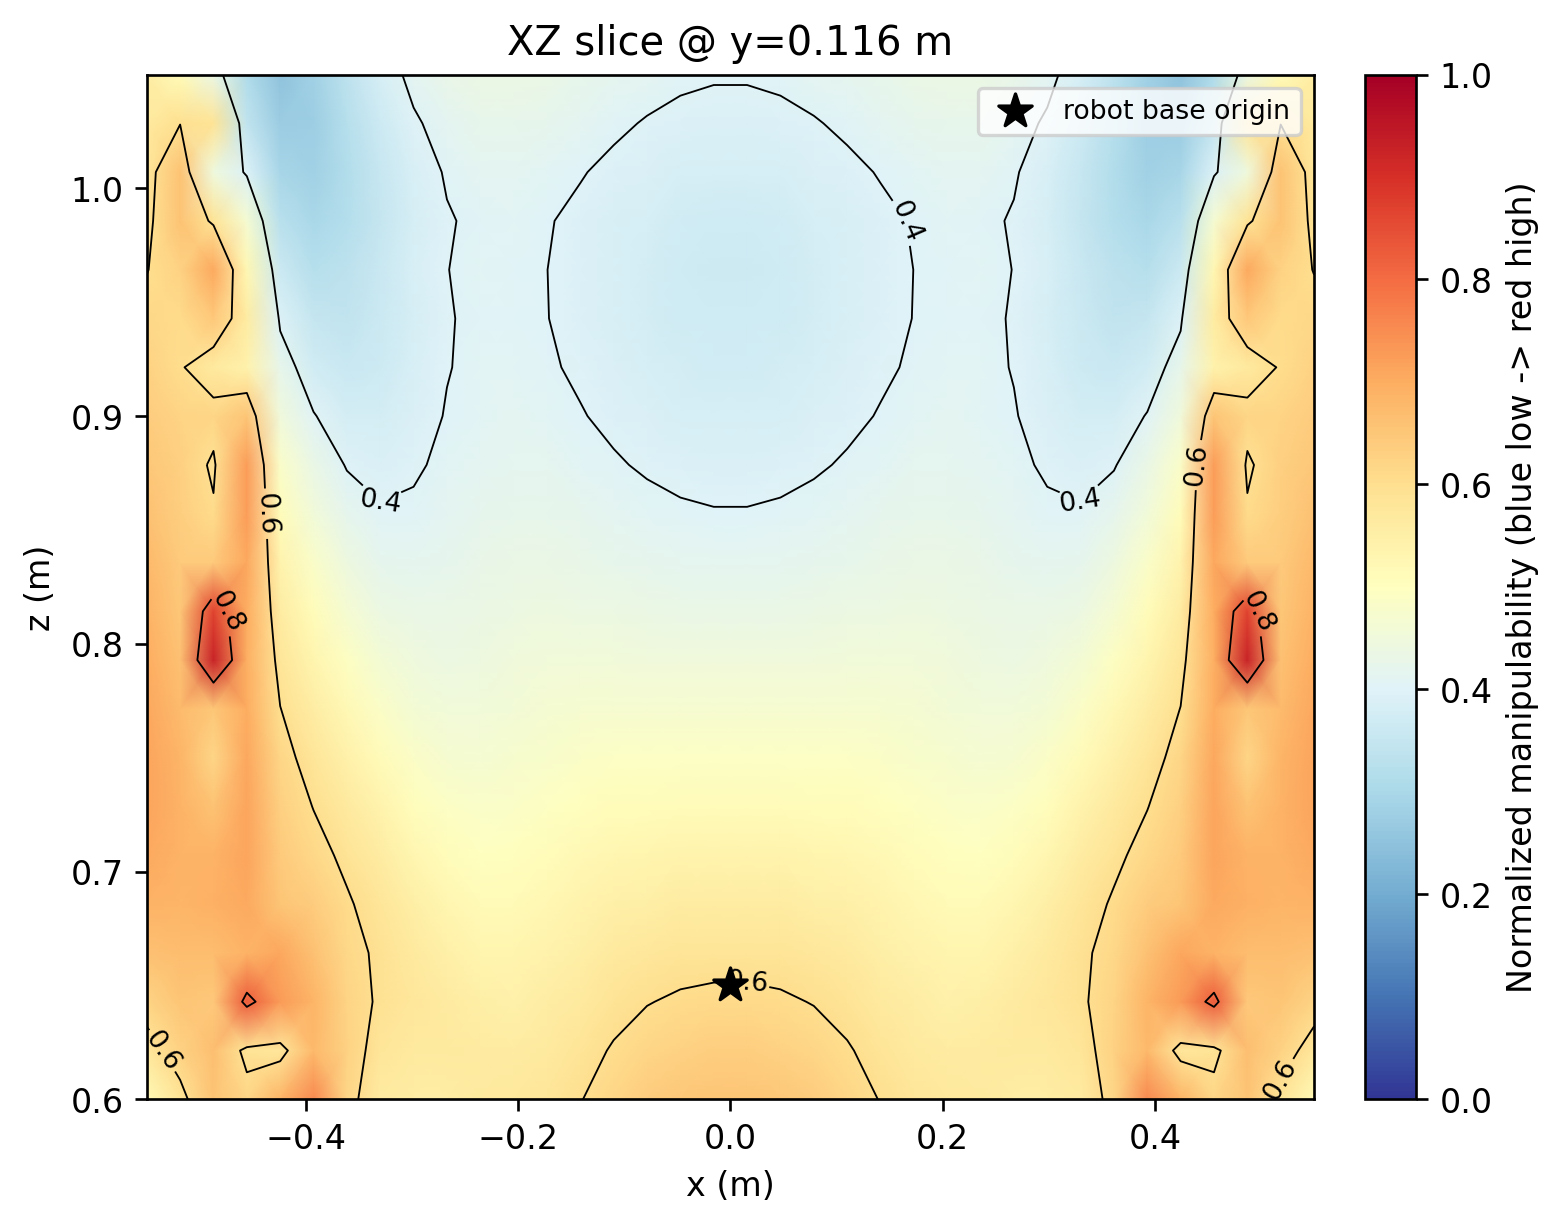
\includegraphics[width=0.24\textwidth]{figures/Manipulability_3.png} &
    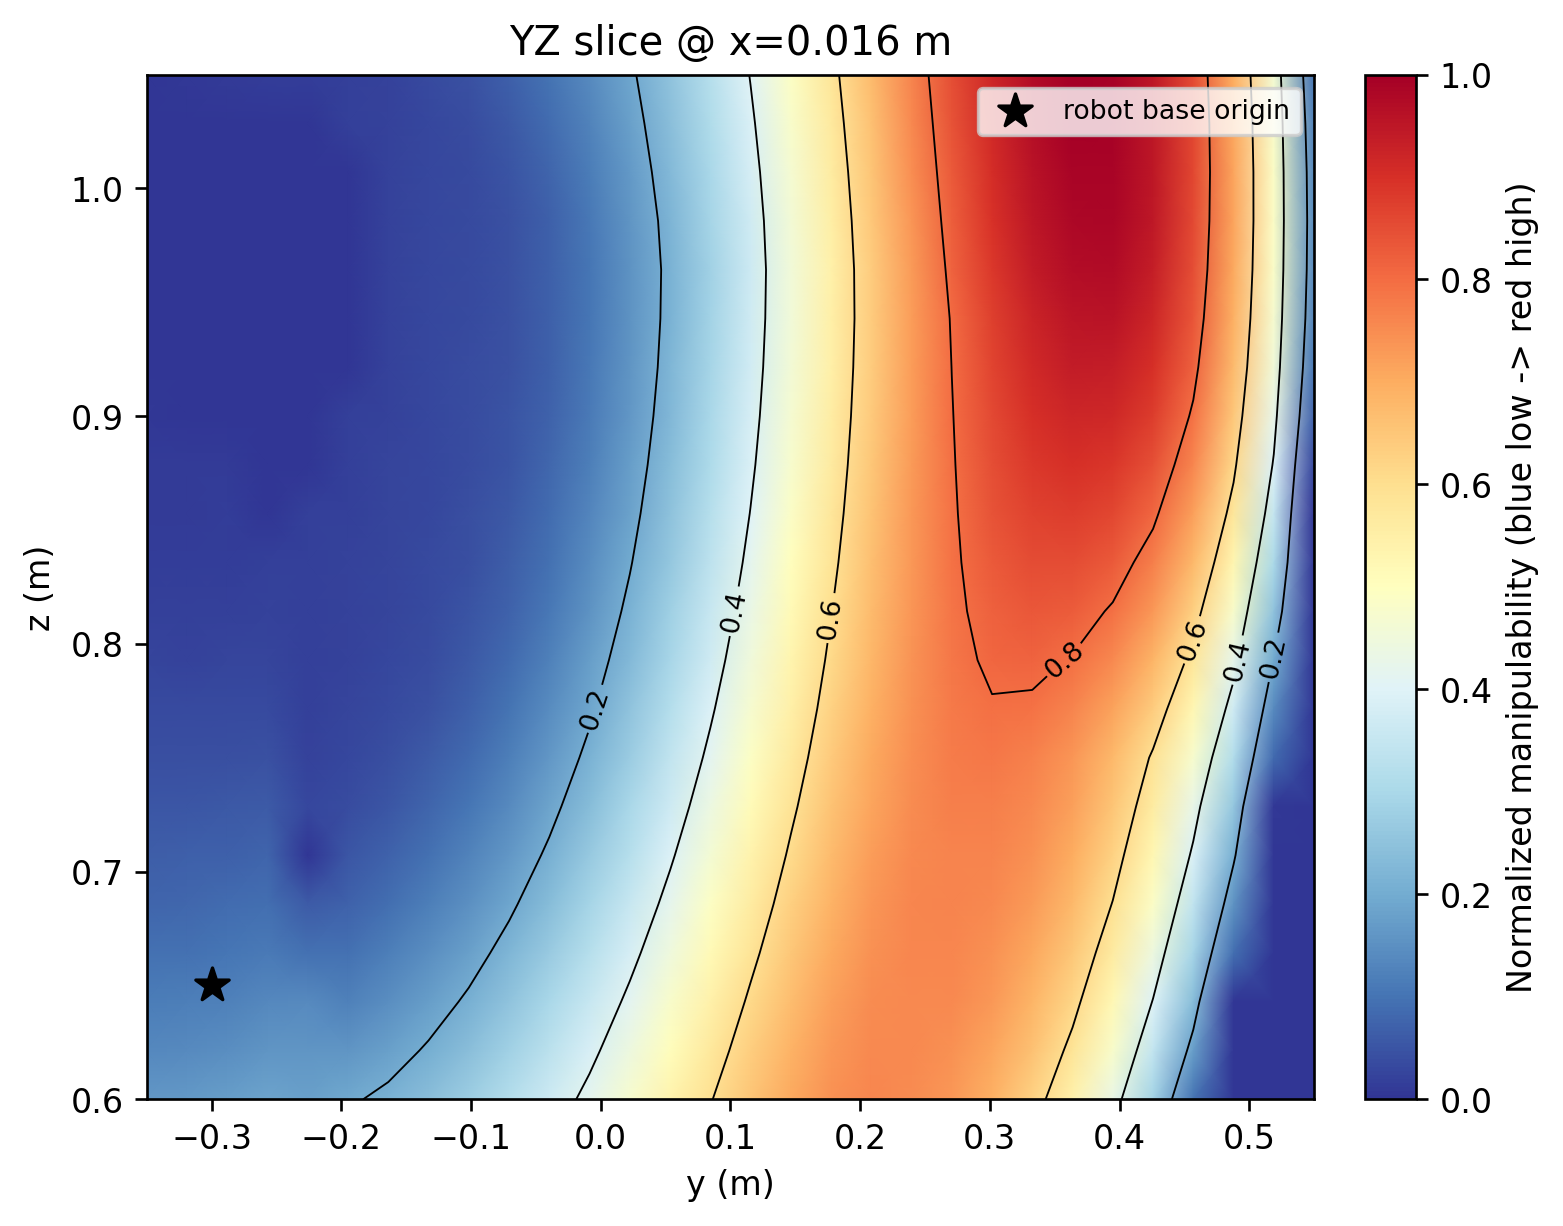
\includegraphics[width=0.24\textwidth]{figures/Manipulability_4.png} \\
    \small (a) & \small (b) & \small (c) & \small (d)
  \end{tabular}
  \caption{Manipulability scores for four candidate object instances: (a) 3D manipulability field, (b)--(d) orthogonal slices. Higher scores indicate more dexterous approach configurations; instances are ranked accordingly for scene-side grounding.}
  \label{fig:manipulability}
\end{figure*}

\subsection{LGP-Based Motion Execution}
\label{sec:motion_execution}

\zz{Introduce in each subsubsection: 1. how LGP is used to solve the motion with active constraints. 2. how motion trajectories are executed on the robot}

Sections~\ref{sec:task_understanding} and~\ref{sec:scene_understanding}
produce two parallel results that must be combined before solving: the task
plan $\mathcal{P}=(B_1,\dots,B_M)$, whose batches specify the structural
slots to be filled (e.g., placing a box-type object on top of an existing
one), and, for each object category, a reachable and manipulability-ordered
list of concrete scene instances. The grounding map $\pi$ of
Section~\ref{sec:problem_formulation} merges the two streams: each structural
slot in the current batch $B_m$ is bound to a concrete instance by scanning
down the ranked candidate list for the required category until a feasible
match is found. This produces a fully grounded batch $\pi(B_m)$, i.e., a list
of concrete object-to-role assignments, which is the input handed to the
solver.

\subsubsection{LGP with Active Constraints}
\textcolor{red}{Input: Action Plans and List of Objects, Output: LGP optimization with active constraints for finding motion trajectories}

Native LGP couples symbolic task structure with continuous trajectory
optimization through a shared representation of predicates, action semantics,
and decision rules~\cite{marc2015LGP}. In principle this abstraction can
solve an assembly task from a symbolic goal alone, but in long-horizon
settings exposing the full generic task domain leads to excessive symbolic
branching and unnecessary geometric backtracking. We therefore instantiate
the native LGP abstraction selectively for each grounded batch $\pi(B_m)$,
compiling only the symbolic relations, object bindings, and decision rules
required by the support pattern active in that batch. The solver thus
receives a grounded symbolic-geometric subproblem tailored to $B_m$ rather
than a monolithic domain covering all possible assembly alternatives.

Discretising a trajectory as $\mathbf{x}_{0:T}=\{x_0,x_1,\dots,x_T\}$ over
$T$ time steps, we keep the native LGP formulation in its original joint
form~\cite{marc2015LGP},
\begin{align}
\min_{\substack{x,\,a_{1:K},\\ s_{1:K},\,t_{1:K}}}\quad
&\int_0^T c\!\left(x(t),\dot{x}(t),\ddot{x}(t)\right)\,dt + \psi\!\left(x(T)\right)
\label{eq:lgp_obj}\\
\text{s.t.}\quad
&\forall k=1{:}K\ \ s_k = \mathrm{succ}(a_k, s_{k-1}),
\label{eq:lgp_succ}\\
&s_K\models g,
\label{eq:lgp_goal}\\
&\forall_{k=1}^{K}\ h_{\mathrm{switch}}\!\left(x(t_k)\mid a_k,s_{k-1}\right)=0,
\label{eq:lgp_sweq}\\
&\forall_{k=1}^{K}\ g_{\mathrm{switch}}\!\left(x(t_k)\mid a_k,s_{k-1}\right)\le 0,
\label{eq:lgp_swineq}\\
&\forall t\in[0,T]\ h_{\mathrm{path}}\!\left(x(t),\dot{x}(t)\mid s_{k(t)}\right)=0,
\label{eq:lgp_patheq}\\
&\forall t\in[0,T]\ g_{\mathrm{path}}\!\left(x(t),\dot{x}(t)\mid s_{k(t)}\right)\le 0,
\label{eq:lgp_pathineq}
\end{align}
where $a_{1:K}$, $s_{1:K}$, and $t_{1:K}$ are the action, symbolic-state, and
switch-time sequences, $g$ is the symbolic goal induced by batch $B_m$, and
$s_k=\mathrm{succ}(a_k,s_{k-1})$ encodes the logic transitions.

For each grounded batch we then solve the corresponding $k$-order Markov
Optimization (KOMO) subproblem in its original constrained sum-of-squares
form~\cite{cite_komo_2014}, i.e., the continuous trajectory-optimization
component of LGP, computing robot and object motions subject to kinematic,
task, and collision constraints:
\begin{align}
\min_{x_{0:T}}\quad
&\sum_{t=0}^{T} f_t\!\left(x_{t-k:t}\right)^\top f_t\!\left(x_{t-k:t}\right)
+\sum_{t,t'} k(t,t')\,x_t^\top x_{t'}
\label{eq:komo}\\
\text{s.t.}\quad
&\forall t:\ g_t\!\left(x_{t-k:t}\right)\le 0,\ h_t\!\left(x_{t-k:t}\right)=0.
\label{eq:komo_c}
\end{align}

The waypoint-level solve also supplies geometric cues that let the downstream
full-motion solve be selective about the collision constraints it
instantiates. Let $x$ denote the full-motion trajectory, $d_{ij}(x)$ the
minimum pairwise distance between collision proxy frames $f_i$ and $f_j$
along $x$, and $f_i^w$ the pose of frame $f_i$ at waypoint $w$. The
trajectory for batch $B_m$ is obtained as
\begin{equation}
x_m^\ast = \arg\min_x J(x),
\label{eq:act_obj}
\end{equation}
subject to collision constraints instantiated only for the active set,
\begin{equation}
c_{ij}(x) = d_{\mathrm{safe}} - d_{ij}(x) \leq 0,
\quad \forall (f_i, f_j) \in \mathcal{C}_{\mathrm{active}}(w),
\label{eq:act_c}
\end{equation}
\begin{equation}
\mathcal{C}_{\mathrm{active}}(w) =
\left\{(f_i, f_j)\ \middle|\ d(f_i^w, f_j^w) < r_{\mathrm{active}}\right\},
\label{eq:act_set}
\end{equation}
where $J(x)$ is the downstream motion objective, $d_{\mathrm{safe}}$ the
prescribed safety margin, and $r_{\mathrm{active}}$ the activation radius
used to screen candidate collision pairs from the waypoint geometry. Only
pairs in $\mathcal{C}_{\mathrm{active}}(w)$ become explicit collision
constraints in the full-motion solve, which reduces unnecessary collision
checks and shortens solve time without altering the structural plan. The
output of this step is the collision-free trajectory $x_m^\ast$ for the
current batch: the decomposition module decides which support relations to
realize next, and native LGP resolves whether and how they can be executed
under the current scene geometry.

\subsubsection{Motion Execution with Joint-Space Impedance Control}
\textcolor{red}{Input: motion trajectories, Output: impedance control for joint torques for motion execution}

Once the trajectory $x_m^\ast$ of a batch is obtained, it is parsed into a
joint-space trajectory and the associated gripper commands and dispatched to
the robot controller for execution on the physical platform. On our Franka
manipulator, the controller tracks the planned joint trajectory through the
arm's built-in joint-space impedance regulation, which converts the tracking
error into joint torques and yields compliant, safe execution at the torque
level; this control layer is a standard property of the platform rather than
a component optimized in this work. The execution layer itself remains
intentionally thin: it streams the planned motion and gripper switches to the
robot and updates the scene state for the next planning--solving cycle, after
which the pipeline proceeds to the following batch $B_{m+1}$.

\section{Results}
\label{sec:results}

\subsection{Experimental Setup and Evaluation Design}
\label{subsec:setup}

\subsection{Necessity of Task Decomposition}
\label{subsec:res_decomp}
% ------------------------------------------------------------------
% FIGURE: fig:ablation_monolithic
% Source data : experiments/outputs/fmb_plots/lgp_combined_results.csv (n=100 raw trials)
% Regenerated : 2026-08-18, aggregated directly from the 100 raw trial_meta.json records at
%               experiments/evaluations/LGP/FMB/3objs/*/trial_*_{nr,r}/lgp_combined/trial_meta.json
% Condition   : FMB, 3 objects (easiest tier), fully-monolithic solving -- NO decomposition at all
%               (neither Smart's active-constraint split nor Global's layer-based split)
% Validity    : recomputed from raw per-trial records on 2026-08-18; independent of the
%               cube-stacking raw-data availability issue noted below (separate eval tree)
% Status      : Leslie-confirmed useful ablation, redrawn 2026-08-18 to fix illegible original
%               (empty scenario labels, cramped runtime subplot)
% ------------------------------------------------------------------
\begin{table}[!ht]
\centering
\caption{Fully-monolithic FMB solving (3 objects, no decomposition): outcome breakdown across all 100 trials, 16GB memory cap and 300s timeout. Motivates decomposition itself, prior to the Smart-vs-Global comparison below.}
\label{tab:ablation_monolithic}
\begin{tabular}{lcccc}
\toprule
Mode & N & Success & Timeout & Mem.-exceeded \\
\midrule
NR & 50 & \phantom{0}0 (0.0\%) & \phantom{0}0 & 50 (100.0\%) \\
R  & 50 & \phantom{0}1 (2.0\%) & 23 (46.0\%) & 26 (52.0\%) \\
\bottomrule
\end{tabular}
\end{table}
\FloatBarrier

\subsection{Direct-Action LLM Baseline is Infeasible}
\label{subsec:res_direct}

\begin{table}[!ht]
\centering
\caption{VLM-MSGraph baseline (Li et al.) execution success rate under Eq.~7 naive straight-line interpolation (no collision checking, no lift/transit/descend decomposition), given the same scenes and task assignment as our method. Task assignment is externally given (from our own method's output), so this isolates the trajectory-generation step.}
\label{tab:baseline_execution}
\begin{tabular}{lcc}
\toprule
 & \multicolumn{2}{c}{Success Rate} \\
\cmidrule(lr){2-3}
Magnitude & NR & R \\
\midrule
\multicolumn{3}{l}{\textit{cubeStacking (N=50 per cell)}} \\
4cubes & 16.0\% & \phantom{0}8.0\% \\
5cubes & \phantom{0}2.0\% & \phantom{0}4.0\% \\
6cubes & \phantom{0}0.0\% & \phantom{0}0.0\% \\
7cubes & \phantom{0}0.0\% & \phantom{0}0.0\% \\
8cubes & \phantom{0}4.0\% & \phantom{0}0.0\% \\
\multicolumn{2}{l}{\textbf{Pooled (N=500)}} & \textbf{3.4\%} \\
\midrule
\multicolumn{3}{l}{\textit{FMB (N=50 per cell)}} \\
3objs & 0.0\% & 0.0\% \\
4objs & 0.0\% & 0.0\% \\
5objs & 0.0\% & 0.0\% \\
\multicolumn{2}{l}{\textbf{Pooled (N=300)}} & \textbf{0.0\%} \\
\bottomrule
\end{tabular}
\end{table}
\FloatBarrier

\subsection{Scalability on Long-Horizon Cube Stacking}
\label{subsec:res_scal}
% ------------------------------------------------------------------
% FIGURE: fig:cube_scalability
% Source data : experiments/outputs/LGP_execution_stats/performance_final_1000tasks.svg
% Generator   : experiments/scripts/generate_final_plots.py (mean-based; eval-dir = LGP_execution/cubeStacking)
% Cross-check : numerically identical to embedded values in success_rate_comparison.svg and
%               solving_time_comparison.svg (independently verified 2026-08-18); matches
%               tab:cube_sr / tab:cube_time in Arxived/main.tex exactly.
% OPEN ITEM   : raw trial_meta.json records behind this run (N=1000) are not currently on this
%               machine (Leslie: on another machine, not yet re-synced as of 2026-08-18). The
%               number is validated by cross-consistency across 3 independently-rendered files
%               plus the previously published table, but not re-derived from raw logs this round.
% Superseded  : experiments/outputs/LGP_execution_stats/plots/{sr,time}_comparison_{nr,r}.svg show
%               a different (lower) Smart success rate -- confirmed 2026-08-18 to be a smaller/
%               earlier run via generate_lgp_plots.py, NOT the same data as this figure. Excluded.
% Regenerate  : python3 experiments/scripts/generate_final_plots.py
% ------------------------------------------------------------------
\begin{table}[!ht]
\centering
\caption{Cube-stacking planning success rate (\%): Smart (ours) vs Global LGP, under no-redundancy (NR) and redundancy (R) conditions. N=1000 tasks total.}
\label{tab:cube_sr}
\begin{tabular}{lcccc}
\toprule
 & \multicolumn{2}{c}{Smart (Ours)} & \multicolumn{2}{c}{Global} \\
\cmidrule(lr){2-3}\cmidrule(lr){4-5}
Cubes & NR & R & NR & R \\
\midrule
4 & 100.0 & 100.0 & 100.0 & 78.0 \\
5 & 100.0 & 100.0 & \phantom{0}96.7 & 56.0 \\
6 & 100.0 & 100.0 & 100.0 & 57.1 \\
7 & 100.0 & 100.0 & \phantom{0}93.3 & \phantom{0}3.7 \\
8 & 100.0 & 100.0 & \phantom{0}60.0 & \phantom{0}0.0 \\
\bottomrule
\end{tabular}
\end{table}

\begin{table}[!ht]
\centering
\caption{Cube-stacking average solving time in seconds over successful trials. Global-R at eight cubes has no successful trial.}
\label{tab:cube_time}
\begin{tabular}{lcccc}
\toprule
 & \multicolumn{2}{c}{Smart (Ours)} & \multicolumn{2}{c}{Global} \\
\cmidrule(lr){2-3}\cmidrule(lr){4-5}
Cubes & NR & R & NR & R \\
\midrule
4 & 28.7 & 23.3 & \phantom{0}26.9 & \phantom{00}31.8 \\
5 & 31.2 & 34.2 & \phantom{0}38.1 & \phantom{00}63.7 \\
6 & 36.8 & 42.8 & \phantom{0}37.2 & \phantom{0}145.9 \\
7 & 40.9 & 57.7 & \phantom{0}69.0 & \phantom{0}295.8 \\
8 & 55.0 & 61.6 & \phantom{0}77.9 & \phantom{0}--- \\
\bottomrule
\end{tabular}
\end{table}


\subsection{Fine-Grained Assembly on FMB}
\label{subsec:res_fmb}
% ------------------------------------------------------------------
% FIGURE: fig:fmb_scalability
% Source data : experiments/outputs/fmb_plots/fmb_success_time_comparison.png
% Generator   : experiments/scripts/generate_fmb_plot.py (mean-based; eval-dir = evaluations/LGP/FMB,
%               N=620 trial_meta.json currently on disk -- fully traceable and reproducible)
% Cross-check : success-rate values closely match tab:fmb_sr; solving-time values closely match
%               tab:fmb_time, EXCEPT the 5-object Global-R bar reads ~15% in this chart vs 6.0%
%               in the Arxived table -- open discrepancy. Leslie decided (2026-08-18) to keep the
%               chart as-is without re-verifying against raw logs this round.
% Regenerate  : python3 experiments/scripts/generate_fmb_plot.py
% ------------------------------------------------------------------
\begin{table}[!ht]
\centering
\caption{FMB planning success rate (\%): Smart (ours) vs Global LGP, under no-redundancy (NR) and redundancy (R) conditions. Scenario-mode groups with 0/N success are excluded from the denominator (affects Global-R at five objects: 3/20 rather than 3/50).}
\label{tab:fmb_sr}
\begin{tabular}{lcccc}
\toprule
 & \multicolumn{2}{c}{Smart (Ours)} & \multicolumn{2}{c}{Global} \\
\cmidrule(lr){2-3}\cmidrule(lr){4-5}
Objects & NR & R & NR & R \\
\midrule
3 & \phantom{0}95.0 & 100.0 & \phantom{0}95.0 & 95.0 \\
4 & \phantom{0}96.7 & \phantom{0}96.7 & \phantom{0}83.3 & 73.3 \\
5 & \phantom{0}98.0 & \phantom{0}98.0 & \phantom{0}66.0 & 15.0 \\
\bottomrule
\end{tabular}
\end{table}

\begin{table}[!ht]
\centering
\caption{FMB average solving time in seconds over successful trials.}
\label{tab:fmb_time}
\begin{tabular}{lcccc}
\toprule
 & \multicolumn{2}{c}{Smart (Ours)} & \multicolumn{2}{c}{Global} \\
\cmidrule(lr){2-3}\cmidrule(lr){4-5}
Objects & NR & R & NR & R \\
\midrule
3 & \phantom{0}74.6 & \phantom{0}68.1 & \phantom{0}82.2 & \phantom{0}95.8 \\
4 & \phantom{0}88.4 & \phantom{0}84.8 & \phantom{0}88.7 & 135.2 \\
5 & 110.8 & 107.9 & 131.0 & 284.8 \\
\bottomrule
\end{tabular}
\end{table}



\subsection{VLM Front-End Graph Generation Accuracy}
\label{subsec:res_vlm_accuracy}

% ------------------------------------------------------------------
% FIGURE: fig:vlm_backbone_selection
% Source data : Arxived/accuracy_bar_chart.svg (converted to PDF 2026-08-18 via cairosvg, no data
%               values changed -- vector re-render only)
% Purpose     : Leslie (2026-08-18): this is the small-scale backbone-selection experiment that
%               justifies choosing Gemini-3-Flash as the VLM front-end -- several candidate models
%               were compared and Gemini-3-Flash was selected based on this result.
% Generator   : NOT FOUND in experiments/scripts/ (per C2 audit, 2026-08-18). Only reference in the
%               repo is test/fmb_VLM_test/evaluate_fmb_vlm_accuracy.py (test dir, ad-hoc). Title text
%               embedded in the SVG reads "Accuracy is computed from extracted FINAL_JSON blocks
%               only" -- this phrasing matches the PRE-canonicalize_graph scripts (see C3 in
%               DATA_VALIDITY_CRITERIA.md), so whether this specific measurement is exposed to the
%               id-ordering bug is UNVERIFIED. Note it may not be the same failure mode either way:
%               this looks like a JSON-extraction/format-compliance check across models, not a
%               graph-equivalence check against a majority-vote reference -- needs confirming.
% OPEN ITEM   : raw values (2026-08-18 read of the SVG) show Gemini-3-Flash at 100.0% (10/10) on
%               "Test-1" but only 30.0% (3/10) on "Test-3", while Qwen3.6-Plus reads 100.0% (10/10)
%               on BOTH Test-1 and Test-3 -- i.e. by these numbers alone Qwen3.6-Plus looks at least
%               as consistent as Gemini-3-Flash. Leslie: please confirm what Test-1/Test-3 represent
%               (different scenarios vs. repeated trials) and reconcile with the "Gemini-3-Flash did
%               well across the board" selection rationale before finalizing the caption below.
% Sampling    : N=10 per model-test cell (per the chart's own counts, e.g. "10/10", "7/10").
% Regenerate  : generator script not located -- flag if you find/recall it, so this can be reproduced.
% ------------------------------------------------------------------
\begin{table}[!ht]
\centering
\caption{Small-scale VLM backbone selection experiment comparing candidate models on FMB graph-generation accuracy, N=10 trials per model-test cell; motivates the choice of Gemini-3-Flash as the VLM front-end used throughout the rest of this section.}
\label{tab:vlm_backbone_selection}
\begin{tabular}{lcc}
\toprule
Model & Test-1 & Test-3 \\
\midrule
Gemini-3-Flash & 100.0\% (10/10) & \phantom{0}30.0\% (3/10) \\
Qwen3.6-Plus   & 100.0\% (10/10) & 100.0\% (10/10) \\
Qwen3.5-Plus   & \phantom{0}70.0\% (7/10) & \phantom{0}50.0\% (5/10) \\
Qwen3.5-Flash  & \phantom{00}0.0\% (0/10) & \phantom{00}0.0\% (0/10) \\
\bottomrule
\end{tabular}
\end{table}
\FloatBarrier



% ------------------------------------------------------------------
% FIGURES: fig:vlm_accuracy_cube_ours, fig:vlm_accuracy_fmb_ours
% Source data : experiments/outputs/gemini_proposed_method/accuracy_analysis/{cubeStacking,FMB}/accuracy_chart.png
% Generator   : experiments/scripts/visualize_gemini_proposed_method_accuracy.py +
%               visualize_gemini_proposed_method_fmb_accuracy.py (2026-08-17, includes the
%               canonicalize_graph id-ordering fix -- see script comments for the bug this fixed)
% GT method   : SELF-REFERENTIAL majority vote across trials (the trial with the highest
%               cross-trial support is treated as the reference answer). NOT externally/manually
%               verified against the source image. Leslie: source doesn't need annotating in the
%               caption, this is an accepted methodological choice, keep raw files for audit trail.
% Regenerate  : python3 experiments/scripts/visualize_gemini_proposed_method_accuracy.py
%               python3 experiments/scripts/visualize_gemini_proposed_method_fmb_accuracy.py
% ------------------------------------------------------------------
\begin{table}[!ht]
\centering
\caption{Our method's VLM graph-generation accuracy vs. majority-vote reference, cube stacking (5 cases per magnitude).}
\label{tab:vlm_accuracy_cube_ours}
\begin{tabular}{lcccc}
\toprule
Magnitude & Cases & Avg. Accuracy & Min & Max \\
\midrule
4cubes & 5 & 100.0\% & 100\% & 100\% \\
5cubes & 5 & 100.0\% & 100\% & 100\% \\
6cubes & 5 & 100.0\% & 100\% & 100\% \\
7cubes & 5 & \phantom{0}98.0\% & \phantom{0}90\% & 100\% \\
8cubes & 5 & \phantom{0}92.0\% & \phantom{0}70\% & 100\% \\
\midrule
Overall & 25 & \phantom{0}98.0\% & & \\
\bottomrule
\end{tabular}
\end{table}

\begin{table}[!ht]
\centering
\caption{Our method's VLM graph-generation accuracy vs. majority-vote reference, FMB (5 cases per magnitude).}
\label{tab:vlm_accuracy_fmb_ours}
\begin{tabular}{lcccc}
\toprule
Magnitude & Cases & Avg. Accuracy & Min & Max \\
\midrule
3objs & 5 & \phantom{0}94.0\% & \phantom{0}70\% & 100\% \\
4objs & 5 & 100.0\% & 100\% & 100\% \\
5objs & 5 & \phantom{0}88.0\% & \phantom{0}70\% & 100\% \\
\midrule
Overall & 15 & \phantom{0}94.0\% & & \\
\bottomrule
\end{tabular}
\end{table}

% ------------------------------------------------------------------
% FIGURE: fig:vlm_accuracy_baseline
% Source data : experiments/outputs/VLM-MSGraph_baseline/accuracy_analysis/visualizations/per_magnitude_descriptive.png
% Generator   : experiments/scripts/visualize_vlm_msgraph_manual_scores.py (2026-08-18)
% GT method   : MANUAL scoring against the source image (Correct=1/Wrong=0). Track 1 protocol --
%               see docs/ops/VLM_MSGRAPH_BASELINE_EXPERIMENT_DESIGN_2026-08-16.md section 4.
%               Small-N by design (baseline comparison track, self-scoring not feasible for this
%               method); Leslie: will re-run against simulation success rate in a later round.
% Sampling    : 8 configs x 5 scenarios x 1 seed, non-redundant only, supplementary track --
%               NOT the paper's core feasibility claim. Reporting rule fixed in advance: pooled
%               accuracy per benchmark only; per-magnitude bars are explicitly non-trend (N=10
%               per cell) -- do not caption these as a degradation curve.
% Pooled      : cubeStacking 92.0% (46/50, Wilson 95% [81.2%,96.8%]); FMB 46.7% (14/30, Wilson 95% [30.2%,63.9%])
% Regenerate  : python3 experiments/scripts/visualize_vlm_msgraph_manual_scores.py
% ------------------------------------------------------------------
\begin{table}[!ht]
\centering
\caption{VLM-MSGraph baseline (Li et al.) semantic/matching-layer accuracy, manually scored against the source image, non-redundant scenarios only. Per-magnitude cells are descriptive only (N=10 each, not a trend); Pooled rows are the reportable statistic, with Wilson 95\% CI.}
\label{tab:vlm_accuracy_baseline}
\footnotesize
\setlength{\tabcolsep}{3pt}
\begin{tabular}{llccc}
\toprule
Benchmark & Magnitude & Correct/N & Accuracy & 95\% CI \\
\midrule
cubeStacking & 4cubes & 10/10 & 100.0\% & \\
cubeStacking & 5cubes & \phantom{0}9/10 & \phantom{0}90.0\% & \\
cubeStacking & 6cubes & \phantom{0}9/10 & \phantom{0}90.0\% & \\
cubeStacking & 7cubes & \phantom{0}9/10 & \phantom{0}90.0\% & \\
cubeStacking & 8cubes & \phantom{0}9/10 & \phantom{0}90.0\% & \\
cubeStacking & \textbf{Pooled} & \textbf{46/50} & \textbf{92.0\%} & 81.2--96.8 \\
\midrule
FMB & 3objs & 8/10 & 80.0\% & \\
FMB & 4objs & 5/10 & 50.0\% & \\
FMB & 5objs & 1/10 & 10.0\% & \\
FMB & \textbf{Pooled} & \textbf{14/30} & \textbf{46.7\%} & 30.2--63.9 \\
\bottomrule
\end{tabular}
\end{table}
\FloatBarrier

\subsection{Physical Execution}
\label{subsec:res_real}

% ------------------------------------------------------------------
% FIGURE: fig:real_cube_stacking
% Source data : Arxived/Cube_Stacking.png
% Content     : real Franka Panda hardware execution -- table of initial scene + robot-execution
%               photo sequences for 4-8 cube stacking assemblies (one row per magnitude).
% Provenance  : pre-existing asset from the earlier paper draft (Arxived/main.tex fig:cube_stacking,
%               where it was captioned as a task-setup figure only); repurposed here 2026-08-18 as
%               physical-execution evidence for subsec:res_real, since it also shows real robot
%               execution frames, not just the initial scene. Leslie: added 2026-08-18.
% ------------------------------------------------------------------
\begin{figure*}[!t]
\centering
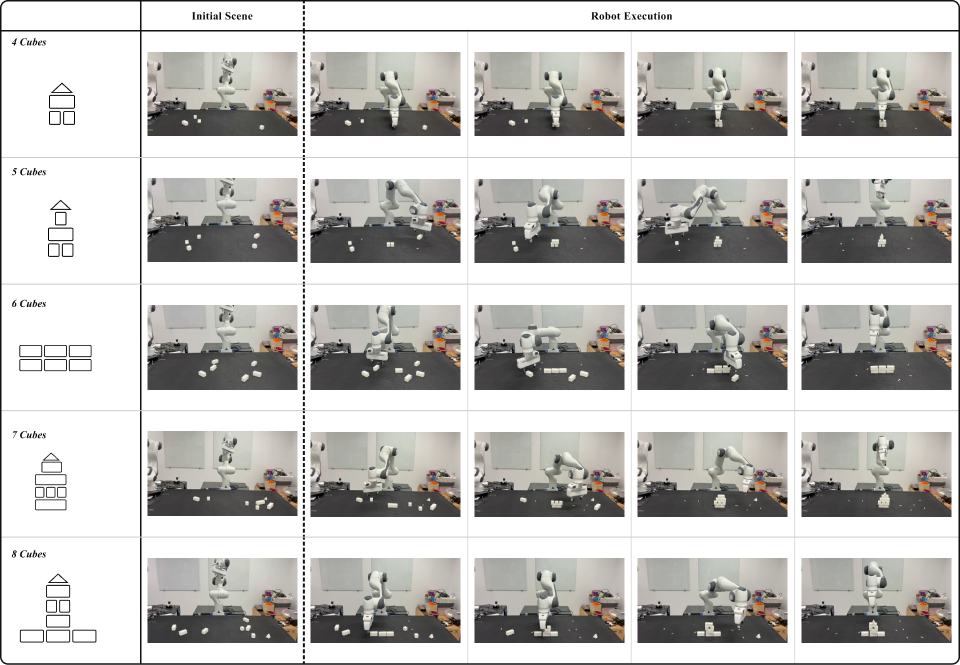
\includegraphics[width=\textwidth]{figures/Cube_Stacking.png}
\caption{Representative real-robot execution: initial scene and execution-sequence photos for cube-stacking assemblies of 4 to 8 cubes on the physical Franka Panda platform.}
\label{fig:real_cube_stacking}
\end{figure*}
\FloatBarrier

% ------------------------------------------------------------------
% FIGURE: fig:real_fmb
% Source data : Arxived/FMB.png
% Content     : real Franka Panda hardware execution -- table of initial scene + robot-execution
%               photo sequences for 3-5 object FMB assemblies (one row per object count).
% Provenance  : pre-existing asset from the earlier paper draft (Arxived/main.tex fig:fmb_overview,
%               where it was captioned as a benchmark-overview figure only); repurposed here
%               2026-08-18 as physical-execution evidence for subsec:res_real, since it also shows
%               real robot execution frames, not just the initial scene. Leslie: added 2026-08-18.
% ------------------------------------------------------------------
\begin{figure*}[!t]
\centering
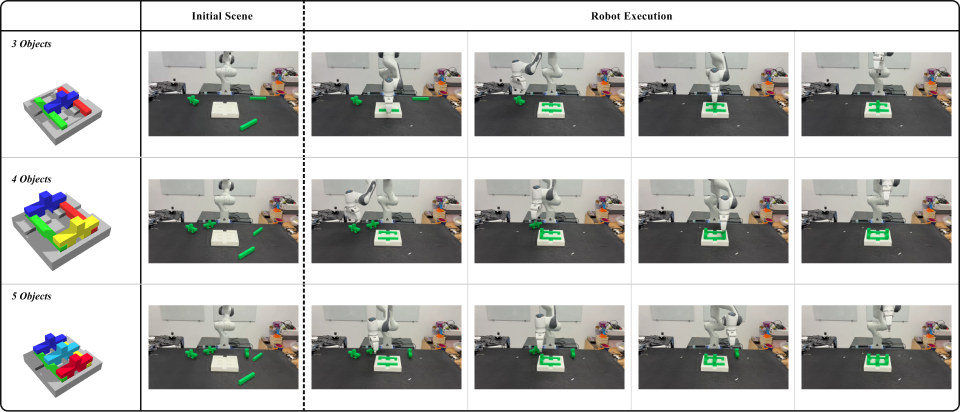
\includegraphics[width=\textwidth]{figures/FMB.png}
\caption{Representative real-robot execution: initial scene and execution-sequence photos for FMB assemblies of 3 to 5 objects on the physical Franka Panda platform.}
\label{fig:real_fmb}
\end{figure*}
\FloatBarrier





\addtolength{\textheight}{-12cm}   % This command serves to balance the column lengths
                                  % on the last page of the document manually. It shortens
                                  % the textheight of the last page by a suitable amount.
                                  % This command does not take effect until the next page
                                  % so it should come on the page before the last. Make
                                  % sure that you do not shorten the textheight too much.



%%%%%%%%%%%%%%%%%%%%%%%%%%%%%%%%%%%%%%%%%%%%%%%%%%%%%%%%%%%%%%%%%%%%%%%%%%%%%%%%
% \section*{APPENDIX}

% Appendixes should appear before the acknowledgment.

% \section*{ACKNOWLEDGMENT}

% The preferred spelling of the word ÒacknowledgmentÓ in America is without an ÒeÓ after the ÒgÓ. Avoid the stilted expression, ÒOne of us (R. B. G.) thanks . . .Ó  Instead, try ÒR. B. G. thanksÓ. Put sponsor acknowledgments in the unnumbered footnote on the first page.



\bibliographystyle{IEEEtran}
\bibliography{ref}



\end{document}
